\FloatBlock
\chapter{Metode}
I dette kapitel beskrives metoderne bag indsamling af data, samt processering af data. Først kommer en beskrivelse af udvælgelse af prøveemner, derefter følger en kort beskrivelse af klassifikationsbestemmelse baseret på en visuel inspection. Derefter følger en beskrivelse af den fotogrammetrisk oppstilling samt efterbehandlig af data anvendt til bulkdensitets bestemmelse, til sidst i kapitlet kommer en beskrivelse af metoden for archimedes princip og opstillingen brugt til bulkdensitets bestemmelse. Alle forsøg udføres i klimakammer ved en temperatur på -6 $\celsius$ ved, DTU - Lyngby. 
%%% ---------- UDVÆLGELSE  AF PRØVEEMNER ---------- %%%
\section{Udvælgelse af prøveemner}
Der bestemmes bulk densitet på 15 prøver, hvilke prøver det er og hvilke boringer de tages fra er forudbestemt. Bulk densitet bestemmelserne ligger til grunde for valg af kerner der på et senere bliver udvalgt oedometer og triaksial -forsøg. 

\noindent Bulkdensiteten bestemmes ved to uafhængige forsøg, i det første forsøg anvendes 3D scanning- struktureret lys metoden, og i det andet forsøg anvendes Archimedes princip, de samme prøveemner anvendes til de to forsøg.

Ved 3D scanningen er der valgt at alle 15 prøver scannes ved en rotationsvinkel på 45 grader, derudover er der udvalgt fire prøver som itlleg scannes ved en rotationsvinkel på 60 og 72 -grader. De fire prøver er udvalgt baseret på visuel inspektion samt masse [g]. 

Formålet ved at anvende forskellige rotationsvinker er å se om vinkelen påvirker resultatet af den afledte densitet. 
I forkant har, test-scanning udføret på DTU-Compute, vist at scannings metoden baseret på struktureret lys har svært ved at håndtere is, af dene grund er der valgt prøver to prøver som antages at have det højeste isindhold af de 15 prøveemner. Derudover er der valgt to prøver der antages at have lavt isindhold.

Derudover er der lagt vægt på at prøveemnerne har samme kernediameter. I prøvepopulationen har 12 prøver en kernediameter på $70 mm$ og tre prøver på $50 mm$. Da det ikke vides på forhånd om prøvens strørrelse har betydning for resultatet af scanningen vælges prøver af samme kernediameter. De fire prøver udvalgt til scanning ved alle rotationsvinkler samt begrundelse, henvises der til tabel \vref{tab:valg_prover}.

%
\begin{table}
\centering
\topcaption{Grundlag for valg af prøveemner til scanning ved alle rotationvinkler, baseret på visuel overflade inspektion samt masse.}
\label{tab:valg_prover}
\begin{tabular}{ll}
\textbf{Prøve} & \textbf{Grundlag/kommentar} \\
\toprule
 B16002\_5B & Ved visuel inspektion vurderes kærnen at have et højt isindhold  \\
 B16004\_3F & Synlig is på prøvens overflade \\
 B16012\_7D & Ingen synlig is, isindhold vurderes til at være lavt \\
 B16019T\_8F & Ingen synlig is, isindhold vurderes til at være lavt \\
\bottomrule
\end{tabular}
\end{table}

\section{Visuel klassifikation}
Klassifikation af prøveemnerne er udført i henhold til standarden (ASTM D4083-89). I klassifikationens standarden er delt op i tre dele: 
Hvor den første del er at afgøre om prøven er frossen eller optøet, denne del beskrives ikke udover dette.

\subsection{Del to} 

Del to omhandler hvordan prøven fremtreder, hvor godt den er bundet sammen og isindholdet. Prøven bliver kategoriseret i hovedgruppen N eller V. Hvor N- dækker over de prøver hvor is ikke kan observeres uden hjelpemidler som f.eks et forstørrelsesglas. Hovedgruppen V -dækker over de prøver hvor segregeret is er synlig for det blotte øje. 


\noindent Ved undergruppering af N-gruppen vurderes der om prøven er velsammenhængende \textbf{Nb}~- intakt, eller \textbf{Nf} - dårlig bundet. Prøverne der kommer i undergruppen \textbf{Nb} inddeles endvidere i to undergrupper: \textbf{Nbn} - intakt og ingen overflødig is eller \textbf{Nbe} -  intakt med overflødig is, for illustration se figur \vref{fig:del2_klass}.

%
\begin{figure}
\centering
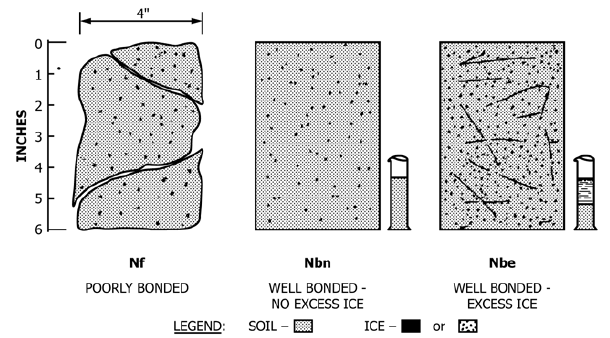
\includegraphics[width=0.6\textwidth]{part1_klass}
\caption{Illustration af de tre kategorier \textbf{Nf},\textbf{Nbn} samt \textbf{Nbe} (ASTM,2007).}
\label{fig:del2_klass}
\end{figure}
%

Prøver der klassifiseres som V deles ind i fem undergrupper- Vx, Vc, Vr, Vs og Vu. Hvor Vx - indikerer individuelle is krystaller eller iklusioner. Vc - indikerer at is fremtreder som belægning på partiklerne. Vr - isformationerne er orienteret tilfældigt eller irregulært. Vs - isformationerne er stratificeret eller tydelig orienteret. Vu - isen er ensartet fordelt, se figur . 
%
\begin{figure}
\centering
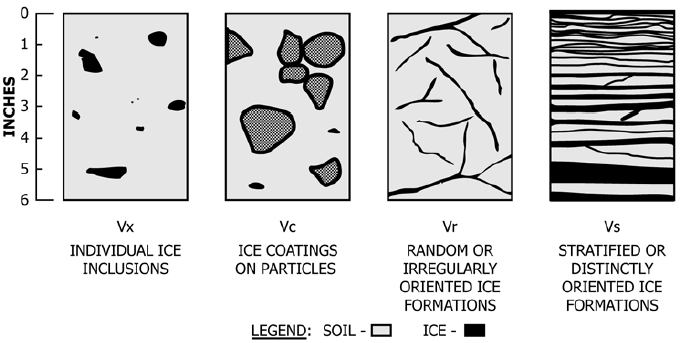
\includegraphics[width=0.6\textwidth]{part1_2_klass}
\caption{Illustration af de fire af de fem underkategorier for prøvens tilstand \textbf{Vx},\textbf{Vc} samt \textbf{Vr} og \textbf{Vs} (ASTM,2007).}
\label{fig:del2_klass}
\end{figure}
%
\subsection{Del tre}
Hvis isstrataen er tykkere en 25 mm som ICE, som deles op i to undergrupper ICE + Soil Type, hvis isinklusionerne indeholder jord og hvis istrataen ikke indeholder jord bliver den tildelt symbolet ICE. 
%%%%%%%

\section{Fotogrammetri- Struktureret lys}
\FloatBlock
Til 3D scanning af prøveemnerne er der anvendt HP 3D Struktureret lys skanner Pro SLS 3, med stereo kamera og rotationsbord.

\noindent Prøverne der scannes er forudbestemt, og er de samme prøver som ved klassifikationen. 
3D scaneren opstilles og kalibreres som beskrevet i bilag \vref{app:3dscan_vejledning}.

% Før prøverne scannes, vejes prøverne tre gange, derefter centreres prøven på rotationsbordet, lys og fokus stilles på kameraerne, se figur \vref{fig:sls_opstilling}. Derefter flyttes prøven og kalibreringspanelet placeres hvor prøven stod \todo[inline,backgroundcolor=anders]{sett inn bilde av kalibreringspanelet}. Ved kalibrering kan det være nødvendig at justere lukketid på de to kameraer samt fokus på både kamera og projektor, dette klaser fra software.

% Efter kalibrering, stilles prøven tilbage, lukketid og fokus stilles, derefter startes scanningen. 
\noindent For skanningen er der valgt tre forskellige rotationsvinkler, se tabel \vref{tab:antal_scans}. Rotationsbordet drejer prøven det valgte antal grader mellem hvert scan. Efter en fuldstendig  360$^{\circ}$ skan, vendes prøven på hovedet og scannes på nyt. Før scanning renses prøven for løst materiale, dette gøres i hånden, derefter vejes prøvens masse. Denne proces gentages inden hver enkelt scanning.

Alle prøver scannes tre gange ved en rotationsvinkel på 45$^{\circ}$. Rotationsvinkelens indflydelse på den beregnede bulkdensitet undersøges ved at fire prøver, scannes tre gange ved rotationsvinkel på 60$^{\circ}$ samt 72$^{\circ}$. De fire prøver der skannes ved 60$^{\circ}$ og 72$^{\circ}$ ses i tabel \vref{tab:prover_60_72}.  
%
\begin{table}
\centering
\topcaption{Rotationsvinkel, og antal skans på 360\degree}
\label{tab:antal_scans}
\begin{tabular}{cc}
\textbf{Vinkel[\degree]} & \textbf{Antal scans}	\\	
\toprule
45	&	8		\\
60	&	6		\\
72	&	5		\\
\bottomrule
\end{tabular}
\end{table}
%
\begin{table}
\centering
\topcaption{Prøve, rotationsvinkel}
\label{tab:prover_60_72}
\begin{tabular}{lcc}
\textbf{Prøve} & \textbf{Grader [\degree]} \\	
\toprule
 B16002\_5B & $60$ & $72$ \\
 B16004\_3F & $60$ & $72$ \\
 B16012\_7D & $60$ & $72$\\
 B16019T\_8F & $60$ & $72$ \\
\bottomrule
\end{tabular}
\end{table}
%

Når alle prøver er scannet en gang (top+bund), ved den givne rotationsvinkel, kalibreres scanneren på nyt og prøverne scannes igen ved samme metode som tidligere angivet. 
Udover de givne 15 prøver er der lavet tre referenceemner, en terning og to cylindre, for terning se figur \vref{fig:terning}, for cylinder 1 se figur \vref{fig:cylinder_1} og for cylinder 2 se figur\vref{fig:cylinder}. De tre referenceemner er scannet for at give et en forståelse af scannerens nøjagtighed. De tre objekters dimensioner målet tre gange med et elektronisk skydelær med en opløsning på 1/10 millimeter. 
Derefter scannes referenceobjekter, tre gange ved en rotationsvinkel på 45$^{\circ}$. Oprindeligt var prøverne hvide, dog var overfladen for blank til at struktureret lys kan anvendes, de ble derfor overfladebehandlet med mat-zinkspray, se figur \vref{fig:zink_spray}.
%
\begin{figure}
\centering
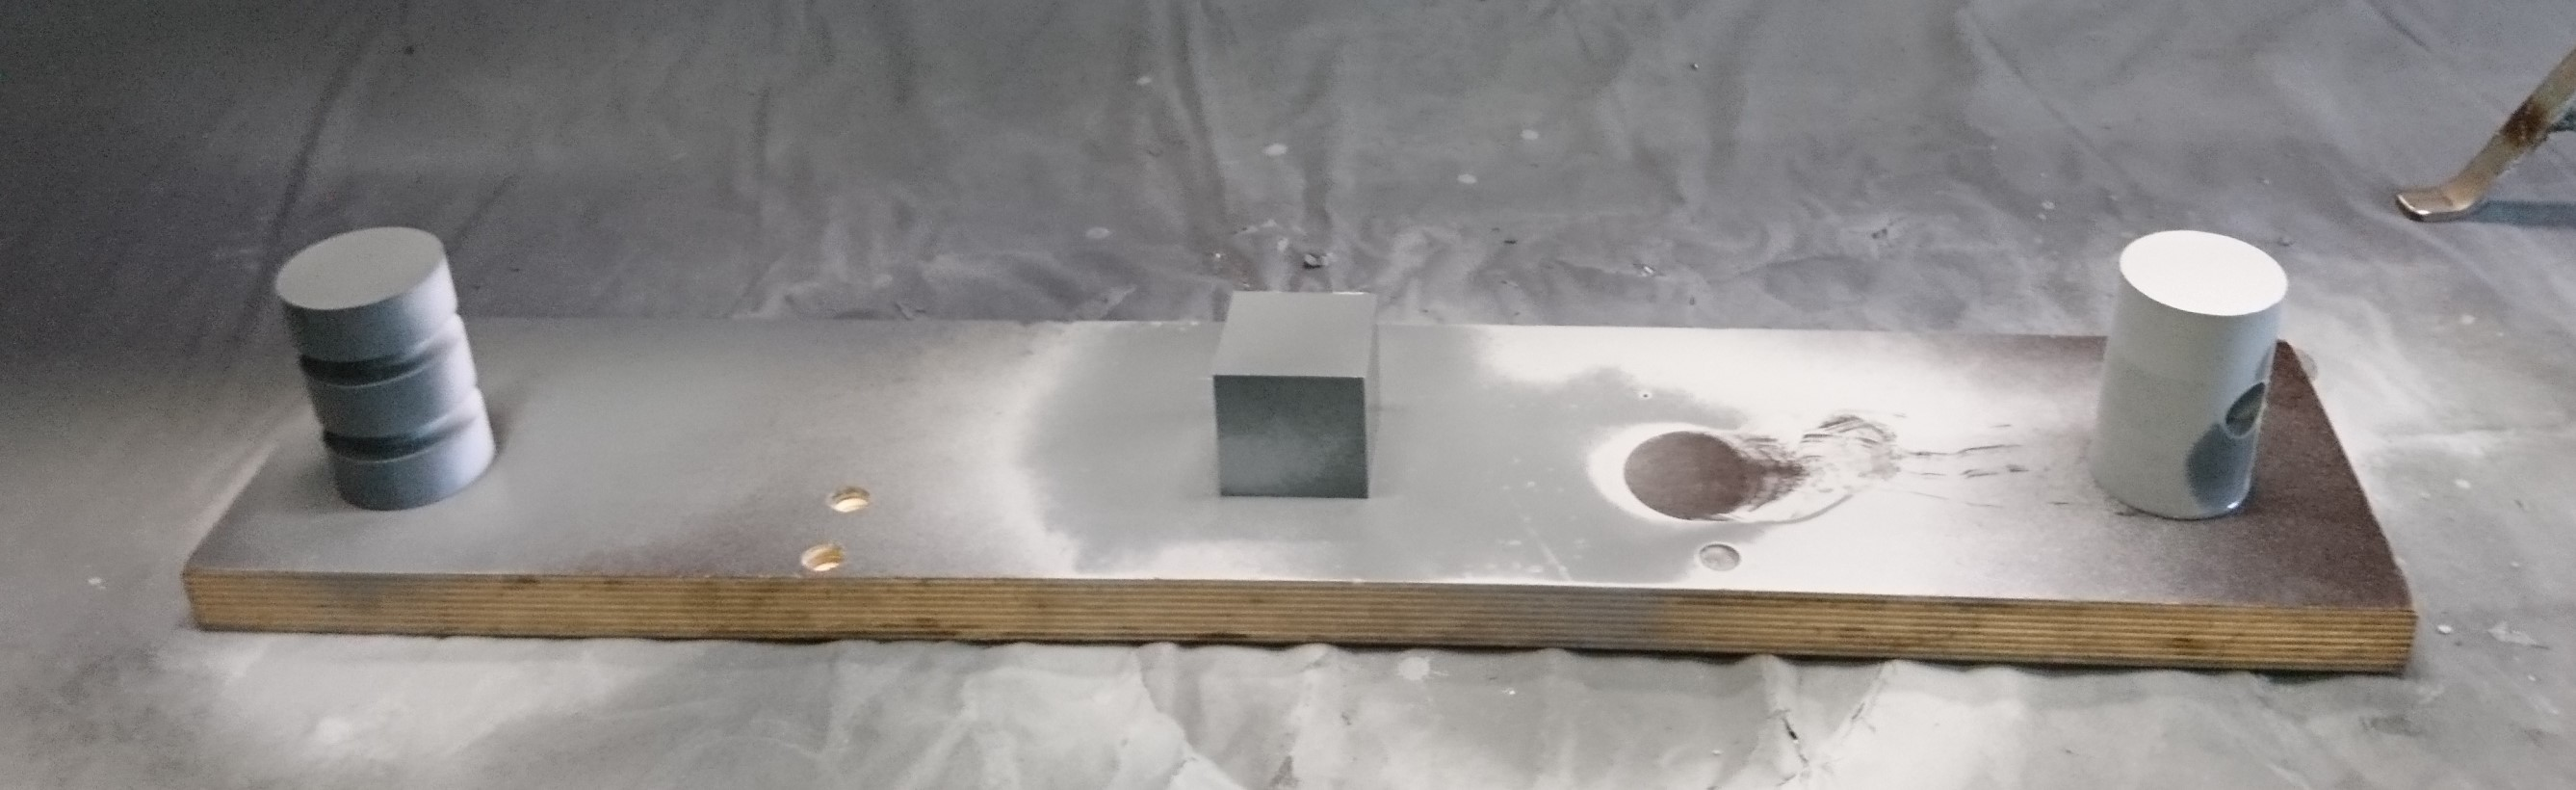
\includegraphics[width=0.6\textwidth]{ref_emner_spray}
\caption{Referenceemnerne gives en mat overflade, med zink spray}
\label{fig:zink_spray}
\end{figure}
%
%
 \begin{figure}
 \centering
 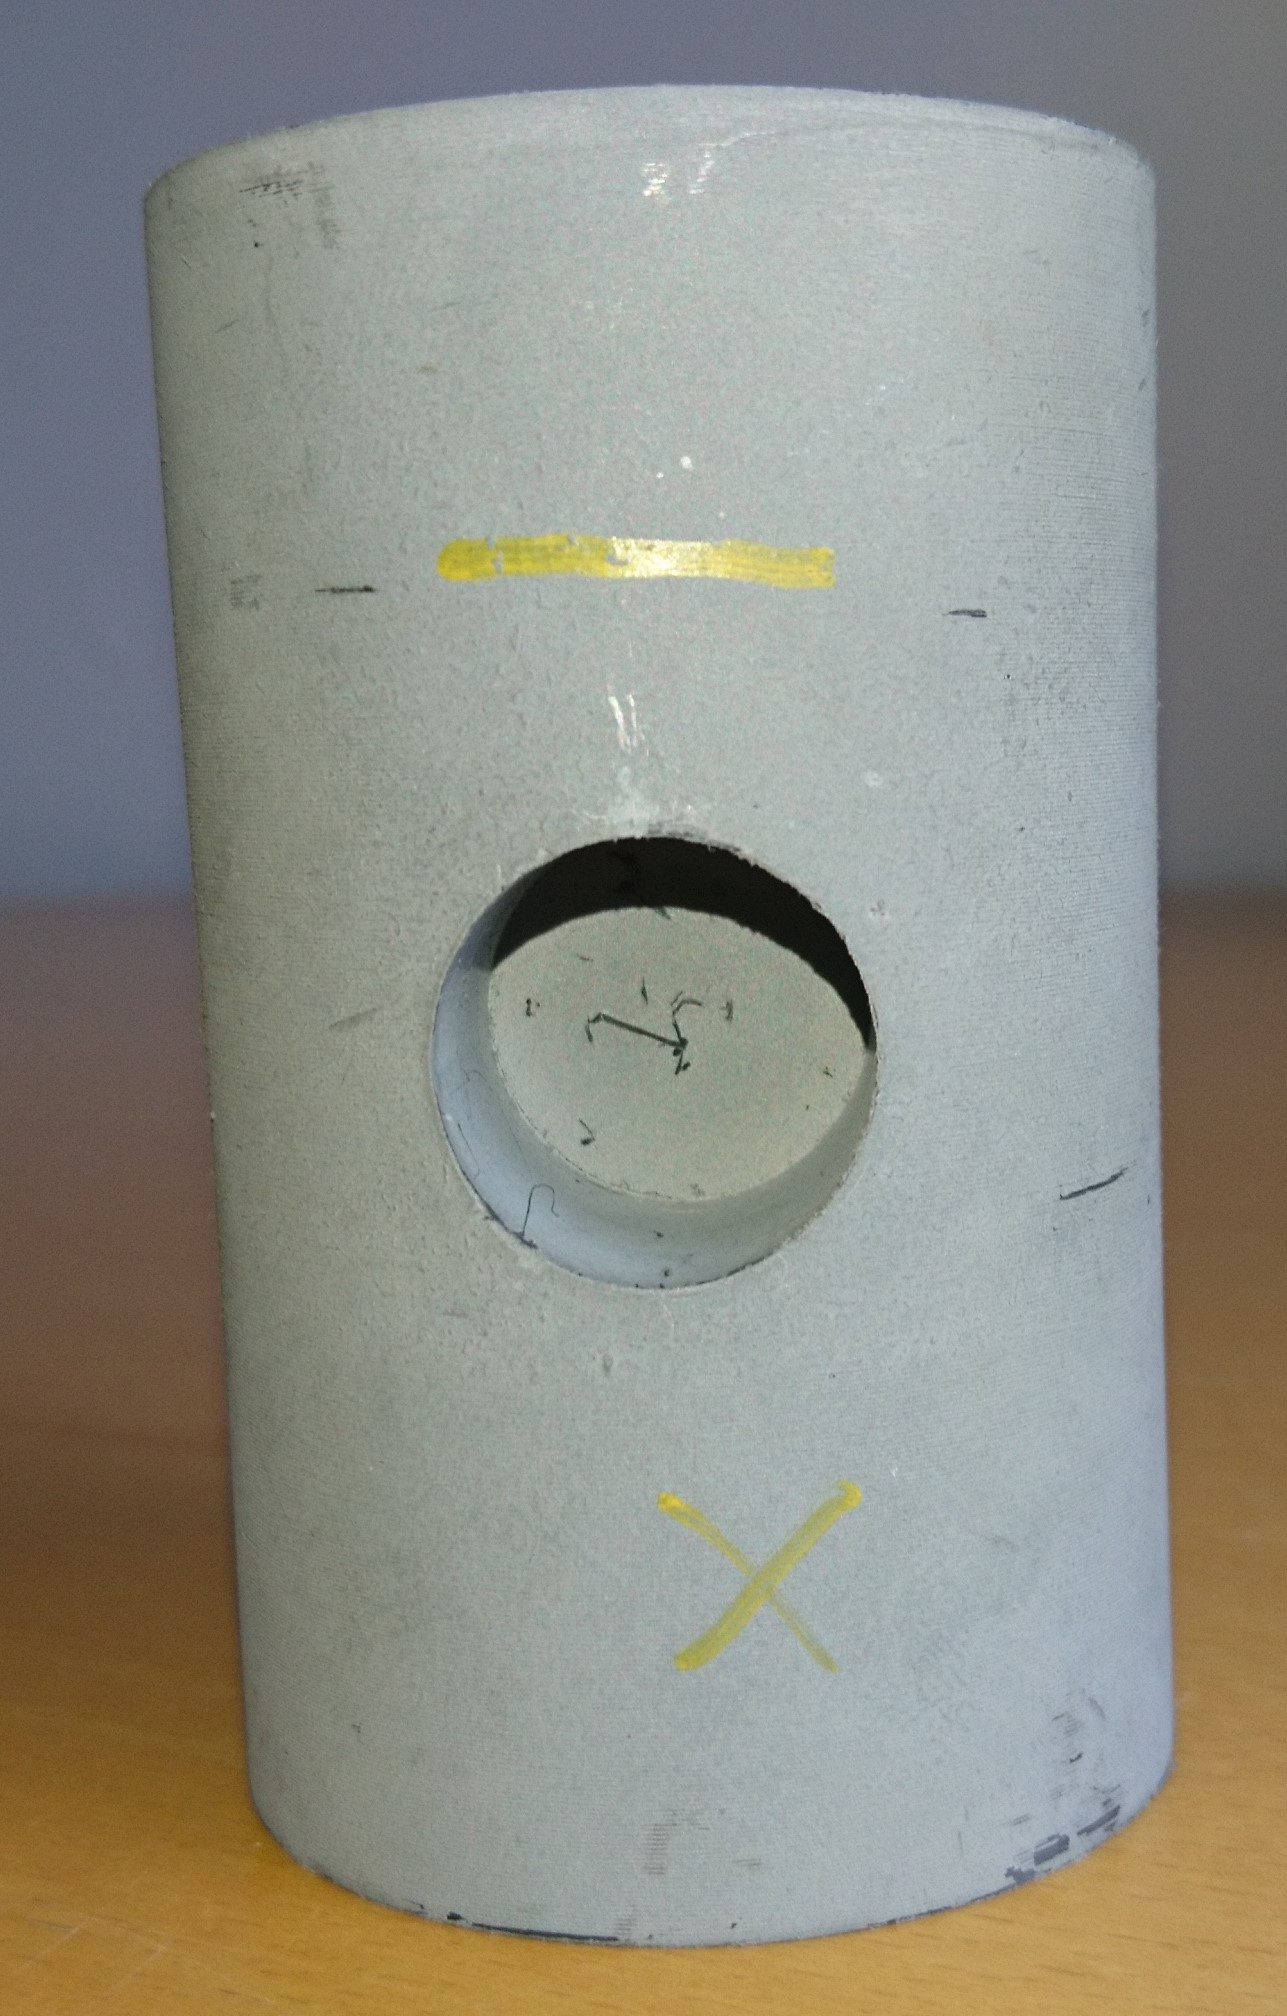
\includegraphics[width=0.3\textwidth]{cylinder_1}
 \caption{Referenceemne - cylinder 1 med dyb indsænkning}
 \label{fig:cylinder_1}
 \end{figure}
%

%
\begin{figure}
\centering
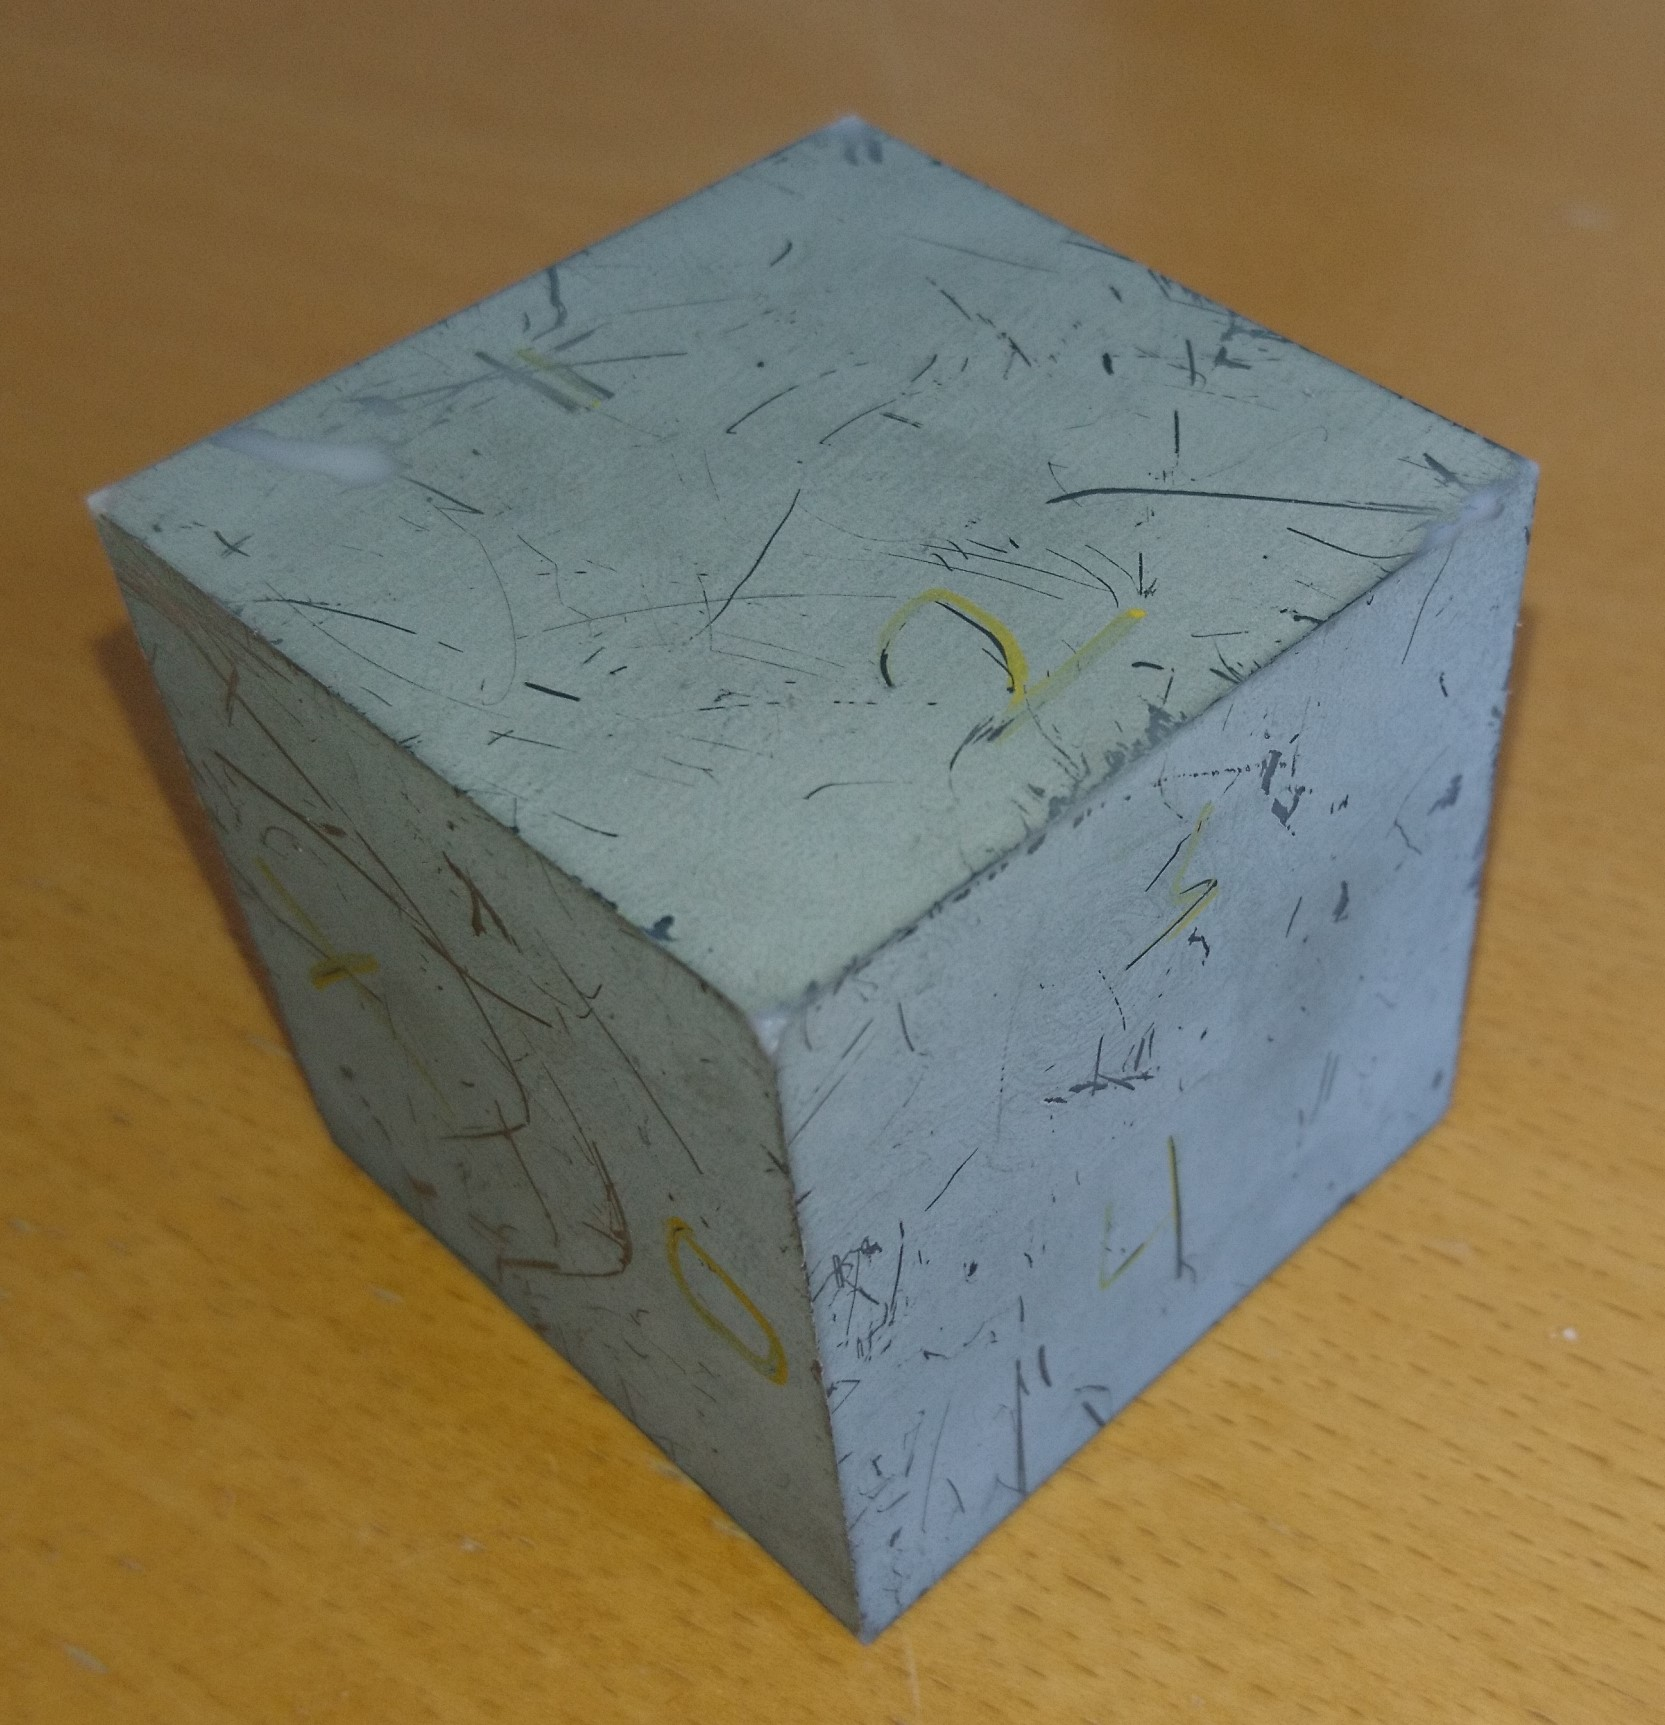
\includegraphics[width=0.4\textwidth]{terning}
\caption{Referenceemne - terning}
\label{fig:terning}
\end{figure}
%
%
\begin{figure}
        \begin{subfigure}[b]{0.45\textwidth}
                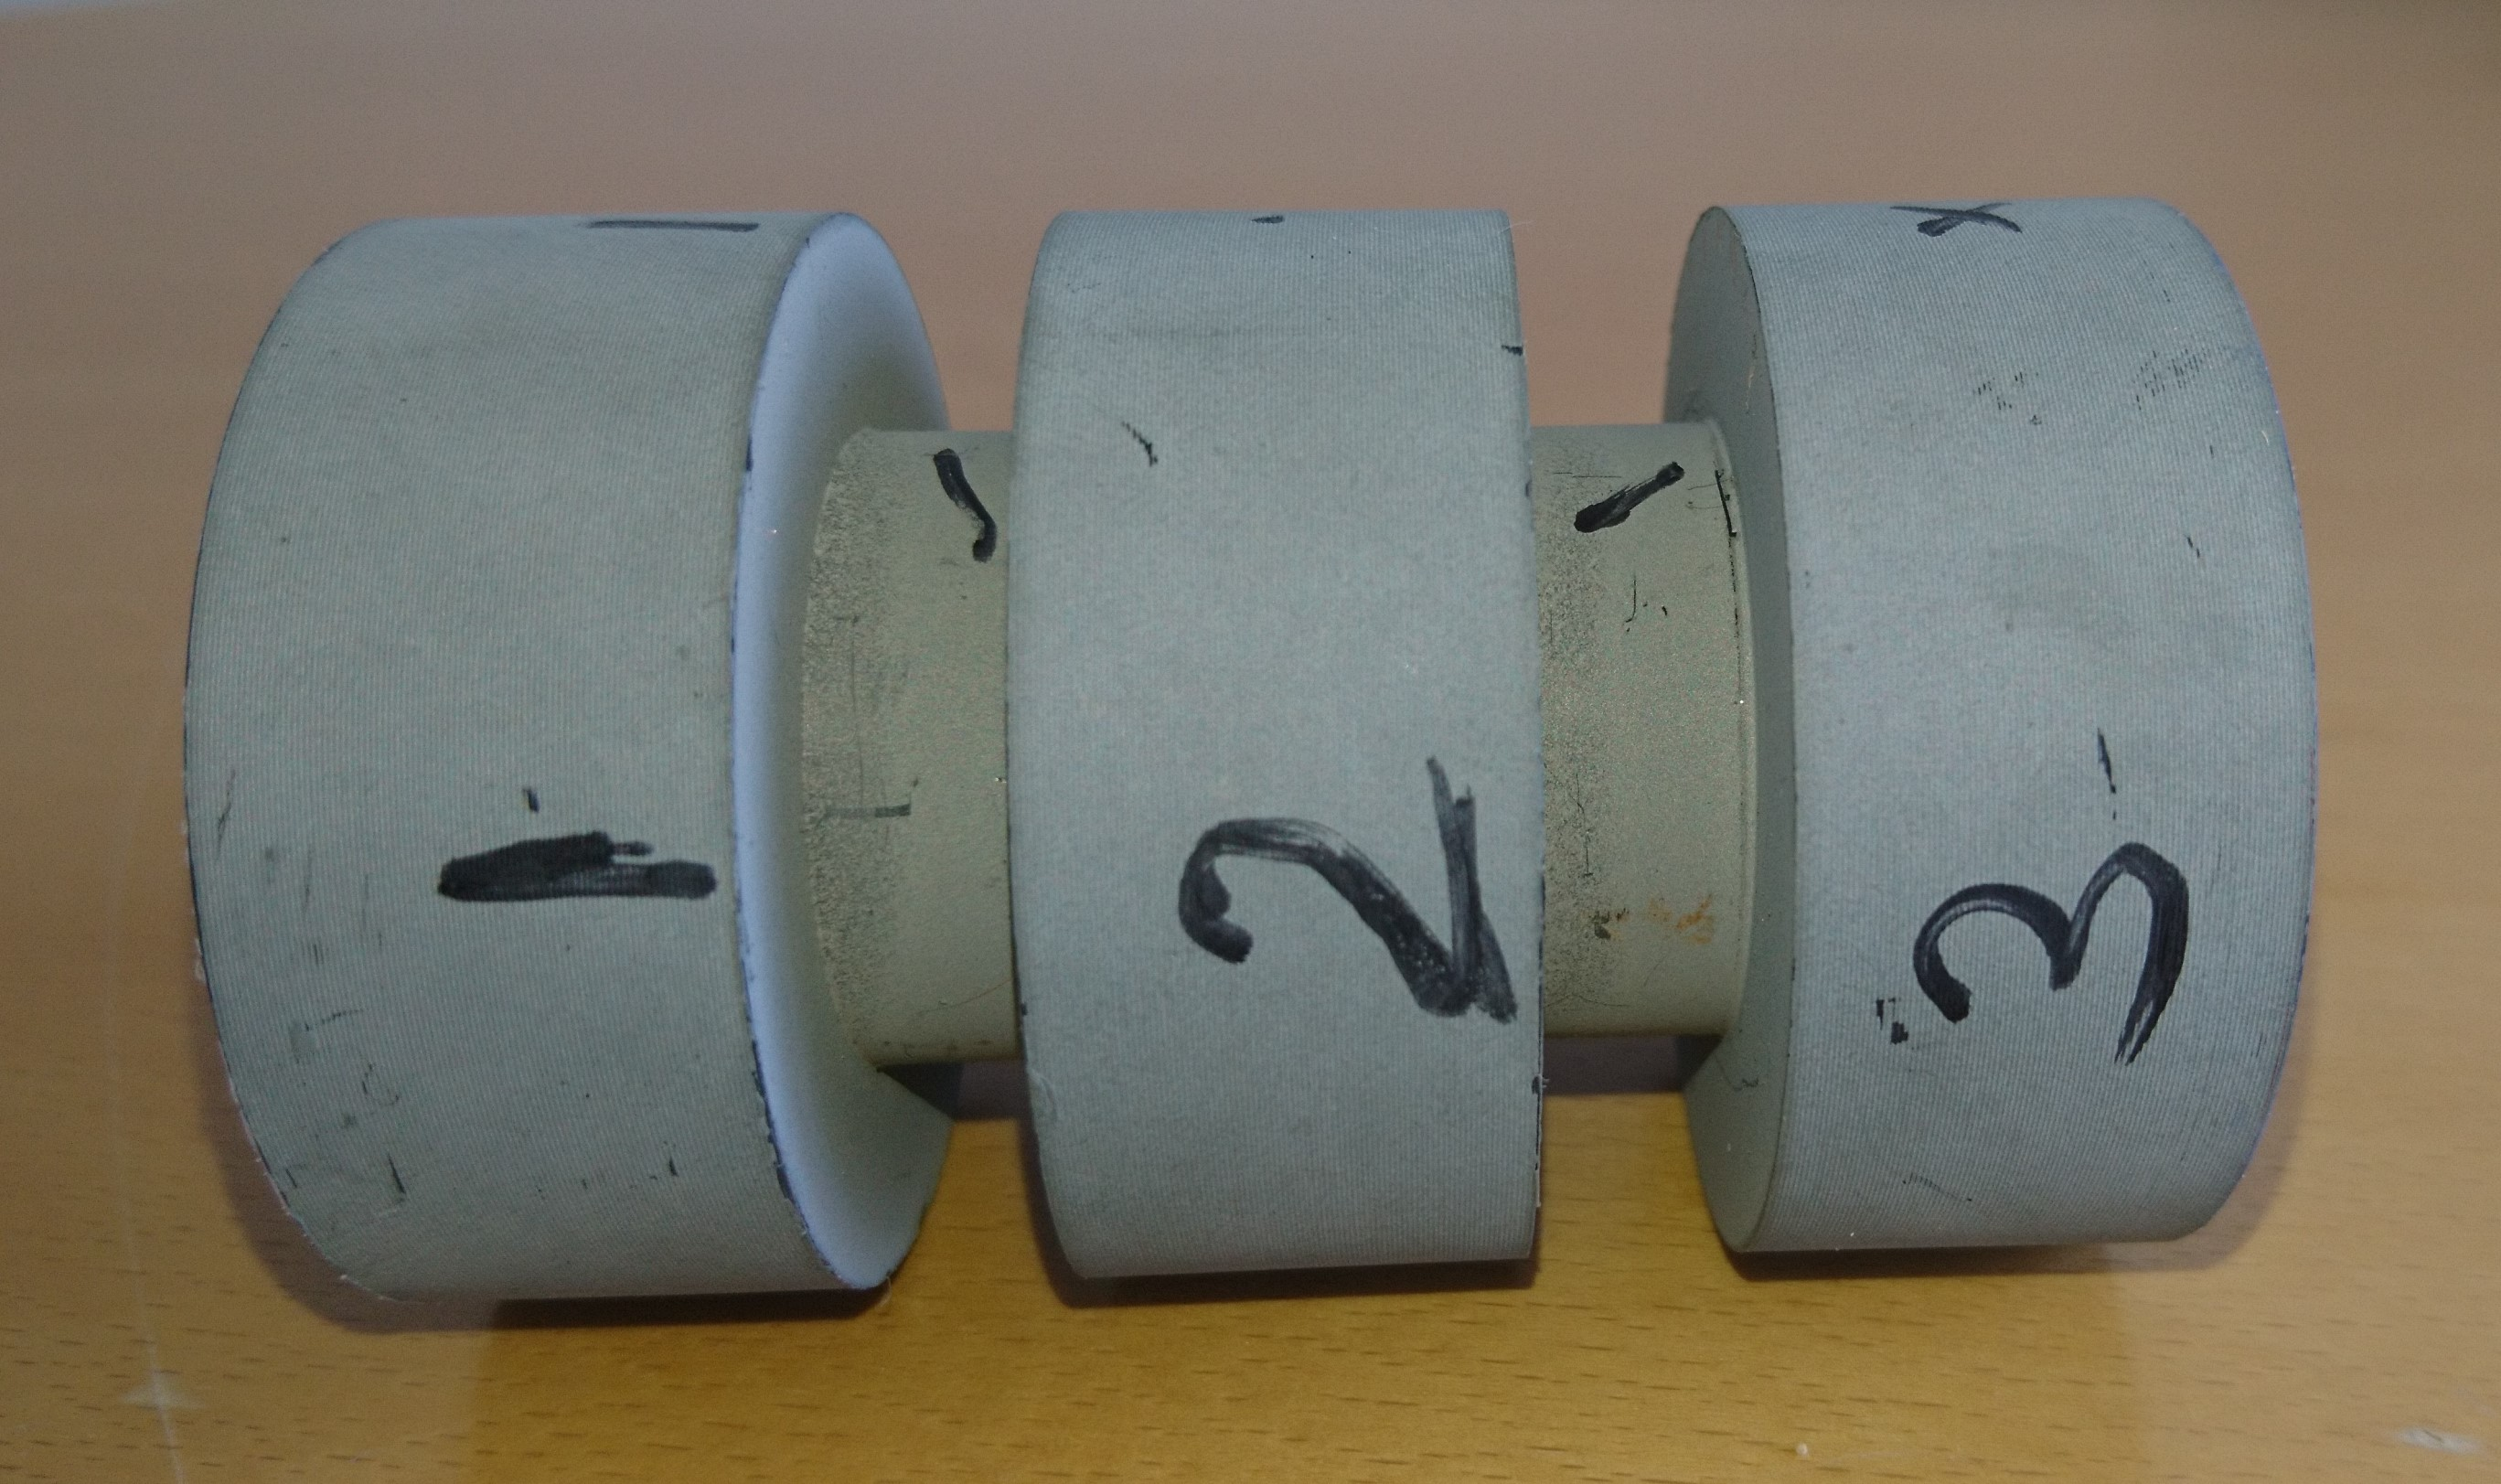
\includegraphics[width=\linewidth]{cylinder_2_2}
                \caption{Cylinder 2 liggende}
                \label{fig:cylinder 2 liggende}
        \end{subfigure}\hfill %
        \begin{subfigure}[b]{0.40\textwidth}
                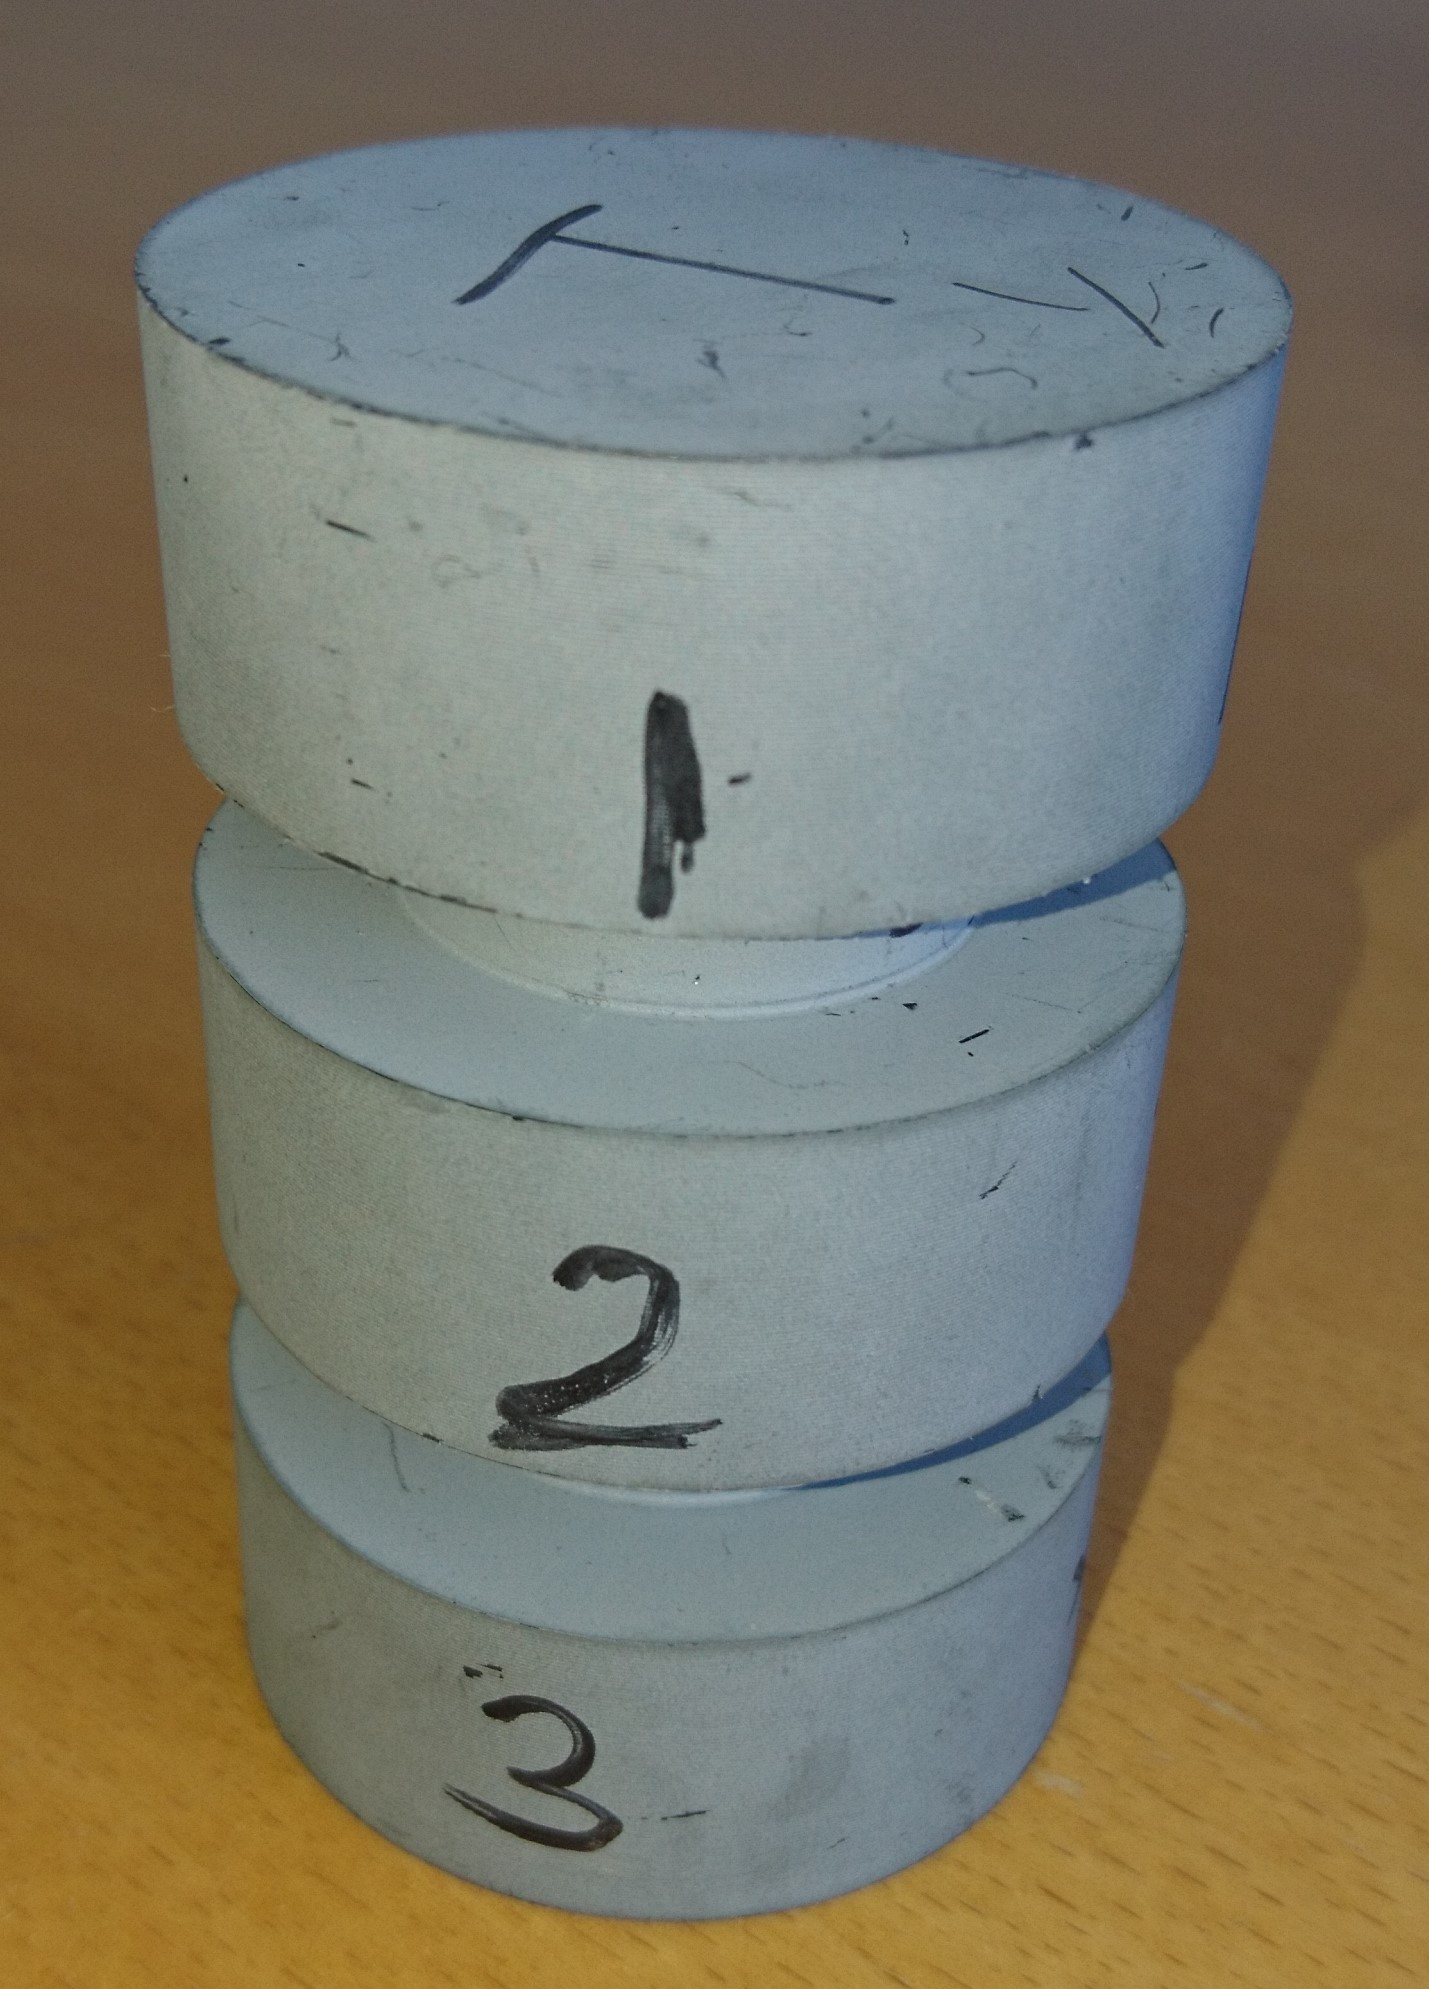
\includegraphics[width=\linewidth]{cylinder_2_3}
                \caption{Cylinder 2 stående}
                \label{fig:cylinder2}
        \end{subfigure}%
        \caption{Referenceemne - cylinder med udfræsninger}\label{fig:cylinder}
\end{figure}
%

Udførelsen af 3D scanning har foregået i frostrummet på DTU, Lyngby, for opstilling se figur \vref{fig:sls_opstilling}. 
%
\begin{figure}
\centering
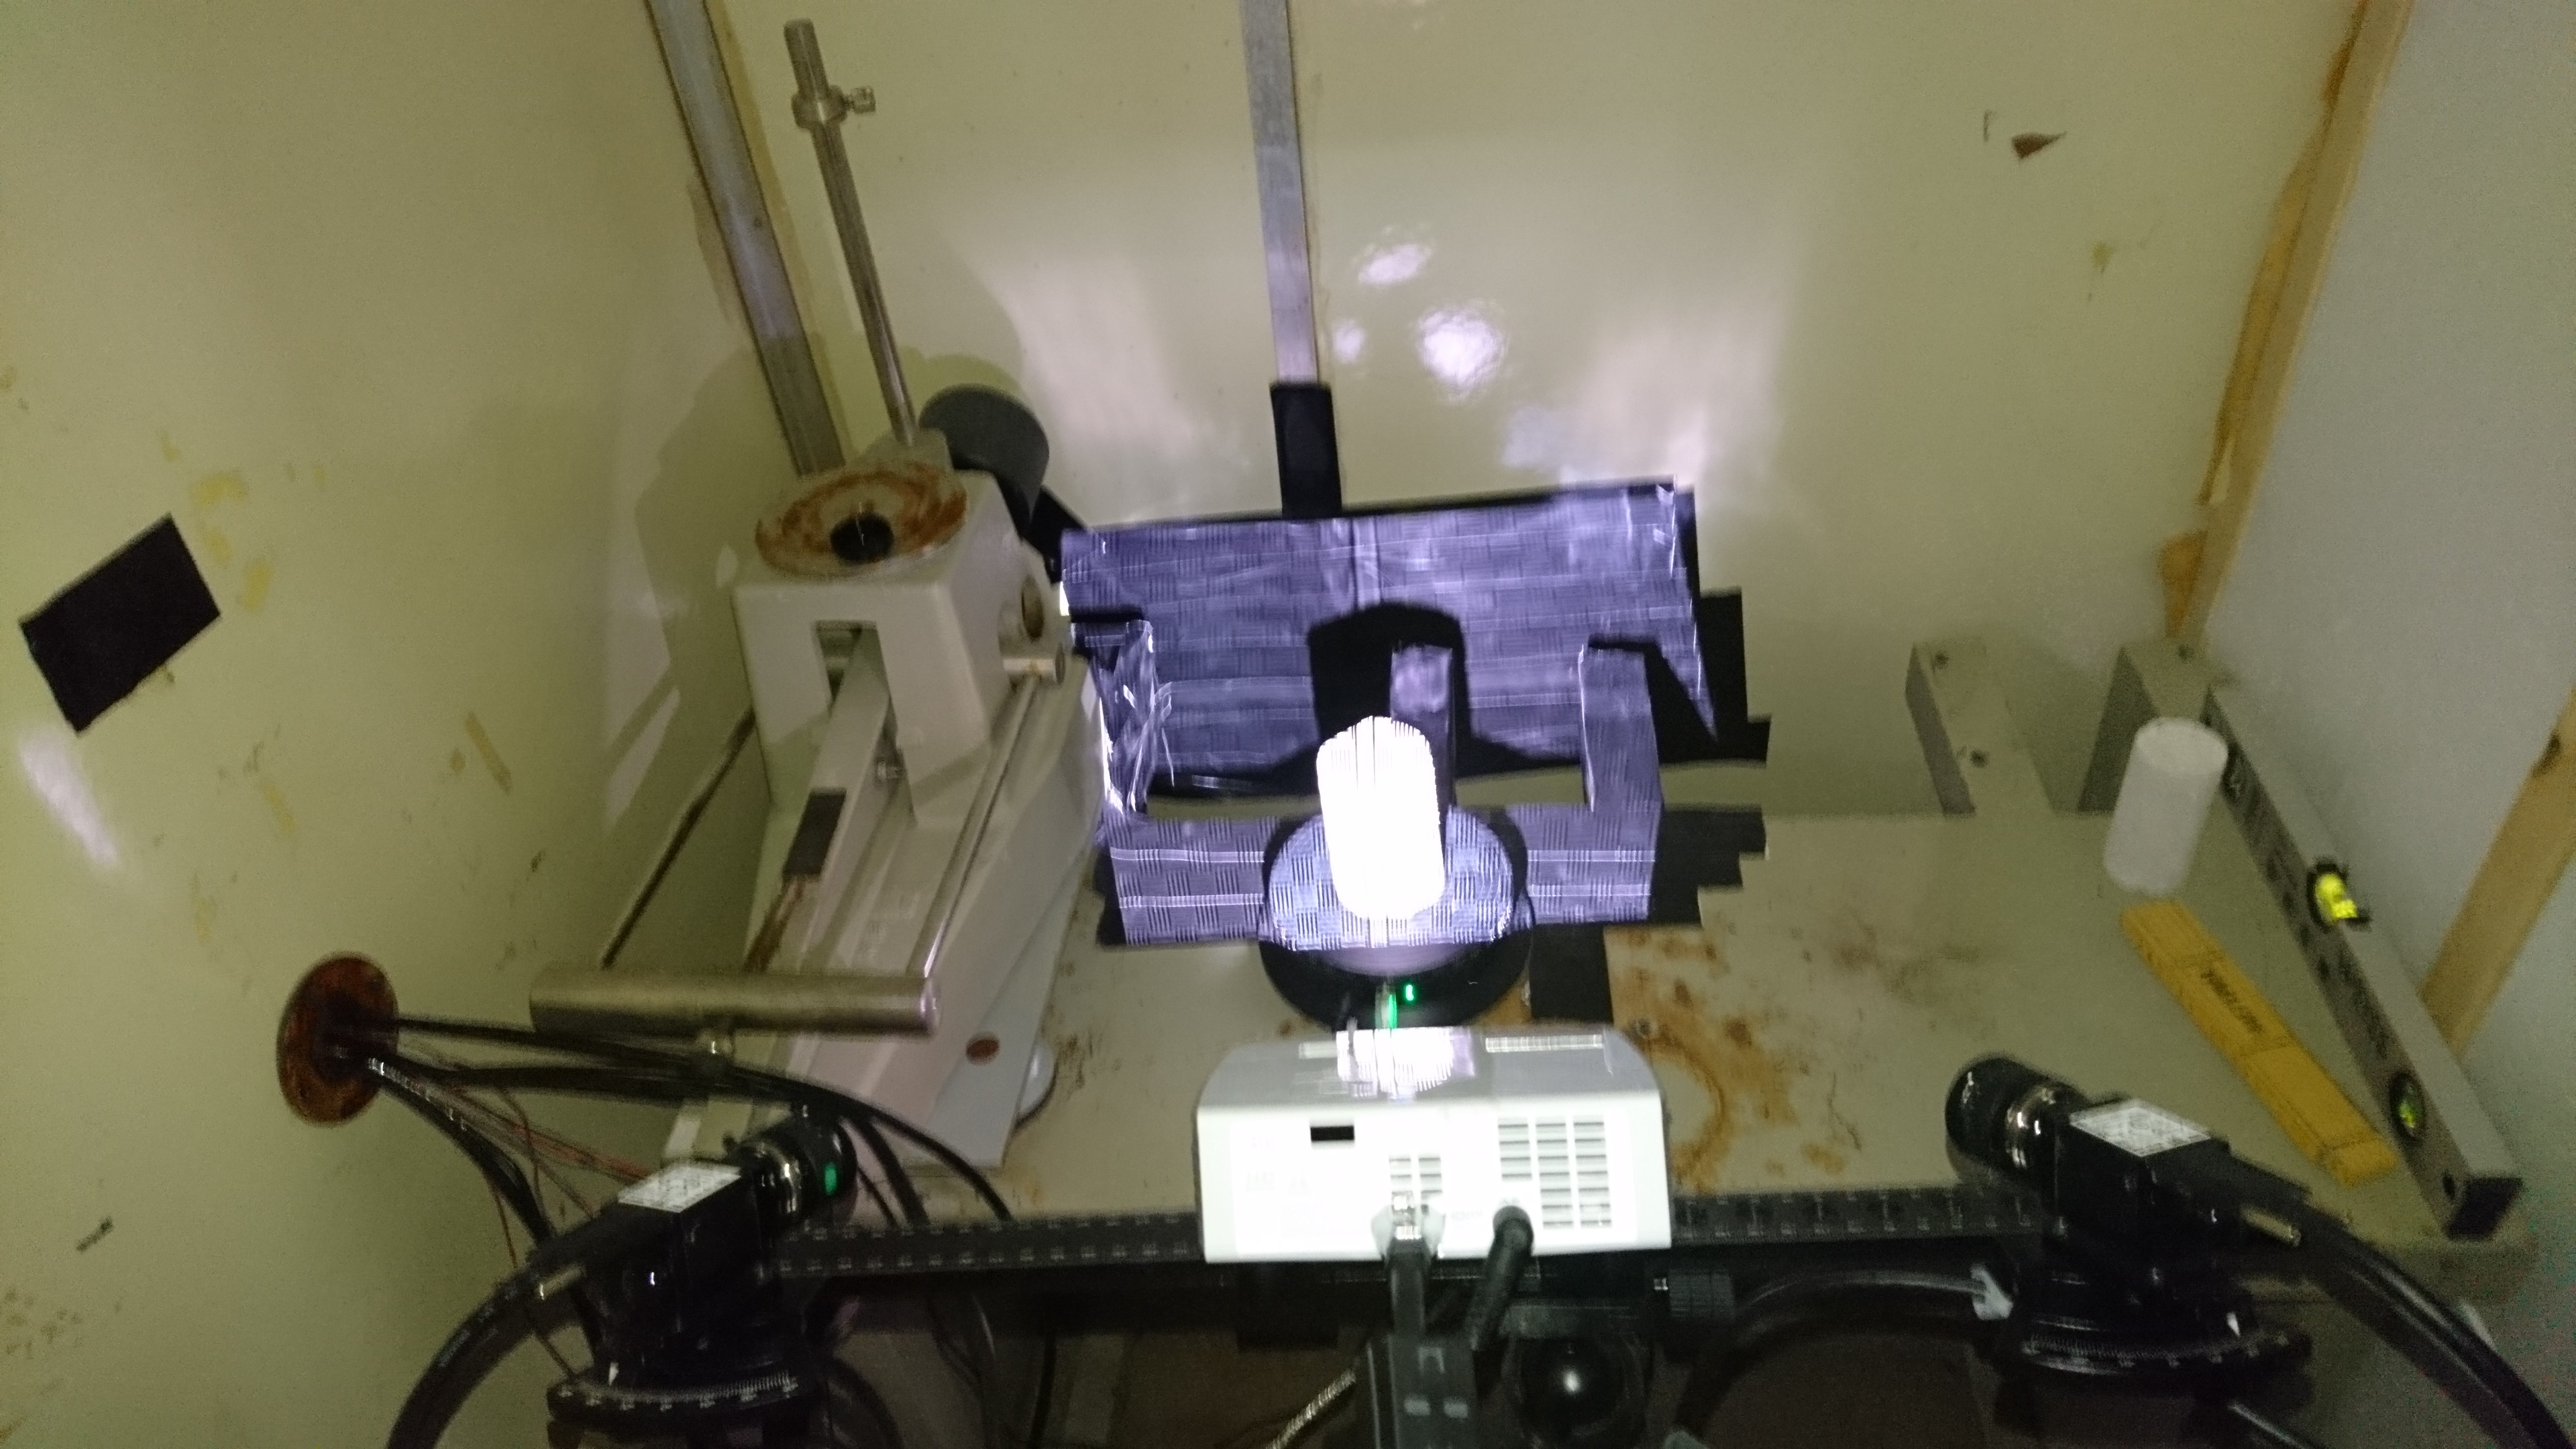
\includegraphics[width=0.7\textwidth]{opstilling_sls_red}
\caption{Prøveopstilling, struktureret lys}
\label{fig:sls_opstilling}
\end{figure}
%

%
%
\noindent Efter alle prøver er scannet, efterbehandles den indsamlede data, som beskrevet i vejledningen se bilag \vref{app:3dscan_vejledning}, og der dannes et vandtæt mesh. 
%
\paragraph{Volumen af mesh} bliver beregnet af to programmer, HP 3D scan og Python. HP 3D scan programmet haver en indebyget funktion der angiver volumen. Til sammenligning er der anvendt Python-modul der kalkulerer volumen af den vandtætte overflade fra stl-fil, til volumen beregning med python anvendes script i separat vedhæftet fil "volumen\_3dscan.py".

\paragraph{Beregning af usikkerhed}
Da de tre scanninger af en prøve er uafhængige af hinanden, masse og volumen kan ændres i mellem hver scanning (m1,m2,m3,v1,v2,v3), bliver m1,v1 osv. parret, og resultatet angives derfor som en middelværdi $\pm$ en spredning. 
Der tages kun højde for den variation der er i densitetsmålingerne, fejlkilder som kan bidrage er vægten, kalibrering af scanner, hvor godt den endelige model passer med punktskyen samt hvordan volumenet beregnes. 
% Til sidst laves der en 3D pdf fremstilling af de 15 prøver der er skannet ved rotationsvinkelen 45$^{\circ}$, samt referenceobjekterne, dette gøres ved at konvertere meshet fra stl- til u3d- format i MeshLab, se separat fil \todo[inline,backgroundcolor=anders]{sett ind navnet på filen}. 
%
\paragraph{Afvigelser fra vejledning:} ved efterbehandling af data blev det konstateret at flere af reference scanningerne ikke var gode nok, pga. den begrensede tidperiode projektet løber over, har der ikke været tid til at lave nye scans af reference emnerne. For at kunne scanne hele fordybningen i cylinder 1 var det nødvendigt at lægge cylinderen vandræt på rotationsbordet, dette medførte problemer ved efterbehandlingen, og det lykkedes ikke at sætte de forskellige scans sammen, af denne grund er forkastes scans og modeller af cylinder 1 og indgår ikke i den videre efterbehandling af resultater. For de to andre referenceemner terning og cylinder 2 kunne der ses i efterbehandlingen at allignment processen ikke blev optimal for de to scanninger, terning 1 og cylinder 2\_1. De har dog blevet vurderet til at være gode nok til den videre efterbehandling.

%%% ---------- Arkimedes princip ---------- %%%
\FloatBlock
\section{Arkimedes princip}
Til den anden del af volumen bestemmelse anvendes Arkimedes princip, hvor prøven neddykkes i en blanding af paraffin og olie (Isopar- L), se datablad i bilag \vref{app:data_isopar}.
Isopar anvendes da forsøget udføres ved en temperatur på $-6${\celsius}.  

\noindent En beholder med Isopar stilles ovenpå en vægte, en separat prøveholder henges op, så den hverken prøveholder eller prøve berører Isopar-beholderens bund eller sider. På prøveholderen festes en temperatur føler. I det følgende anvendes følgende notation: Isopar- I, prøveholder H, vægt/lod - V og prøve - P.

Densiteten af Isopar-L er afhængig af temperaturen, af denne grund bestemmes densiteten af Isopar ved målinger af et lod med et kendt volumen og masse. 

\subsection{Kalibrering af temperaturfølere}
Til måling af temperatur (luft og Isopar) anvendes der datalogger med en opløsning på $0,1${\celsius}. Det anvendte kalibreringsbad til nulpunktskalibrering  er " Fluke 7320" se figur \vref{fig:kalibad}. De tre temperatursensorer festes til metal gitteret, og nedsænkes i kalibrerings-badet. Inden forsøgsstart kalibreres temperaturlogger med computer tid (tt:mm:ss), armbåndsuret til at notere tidspunkt for hver måling inde i frostrummet kalibreres efter computeren.

%
\begin{figure}
\centering
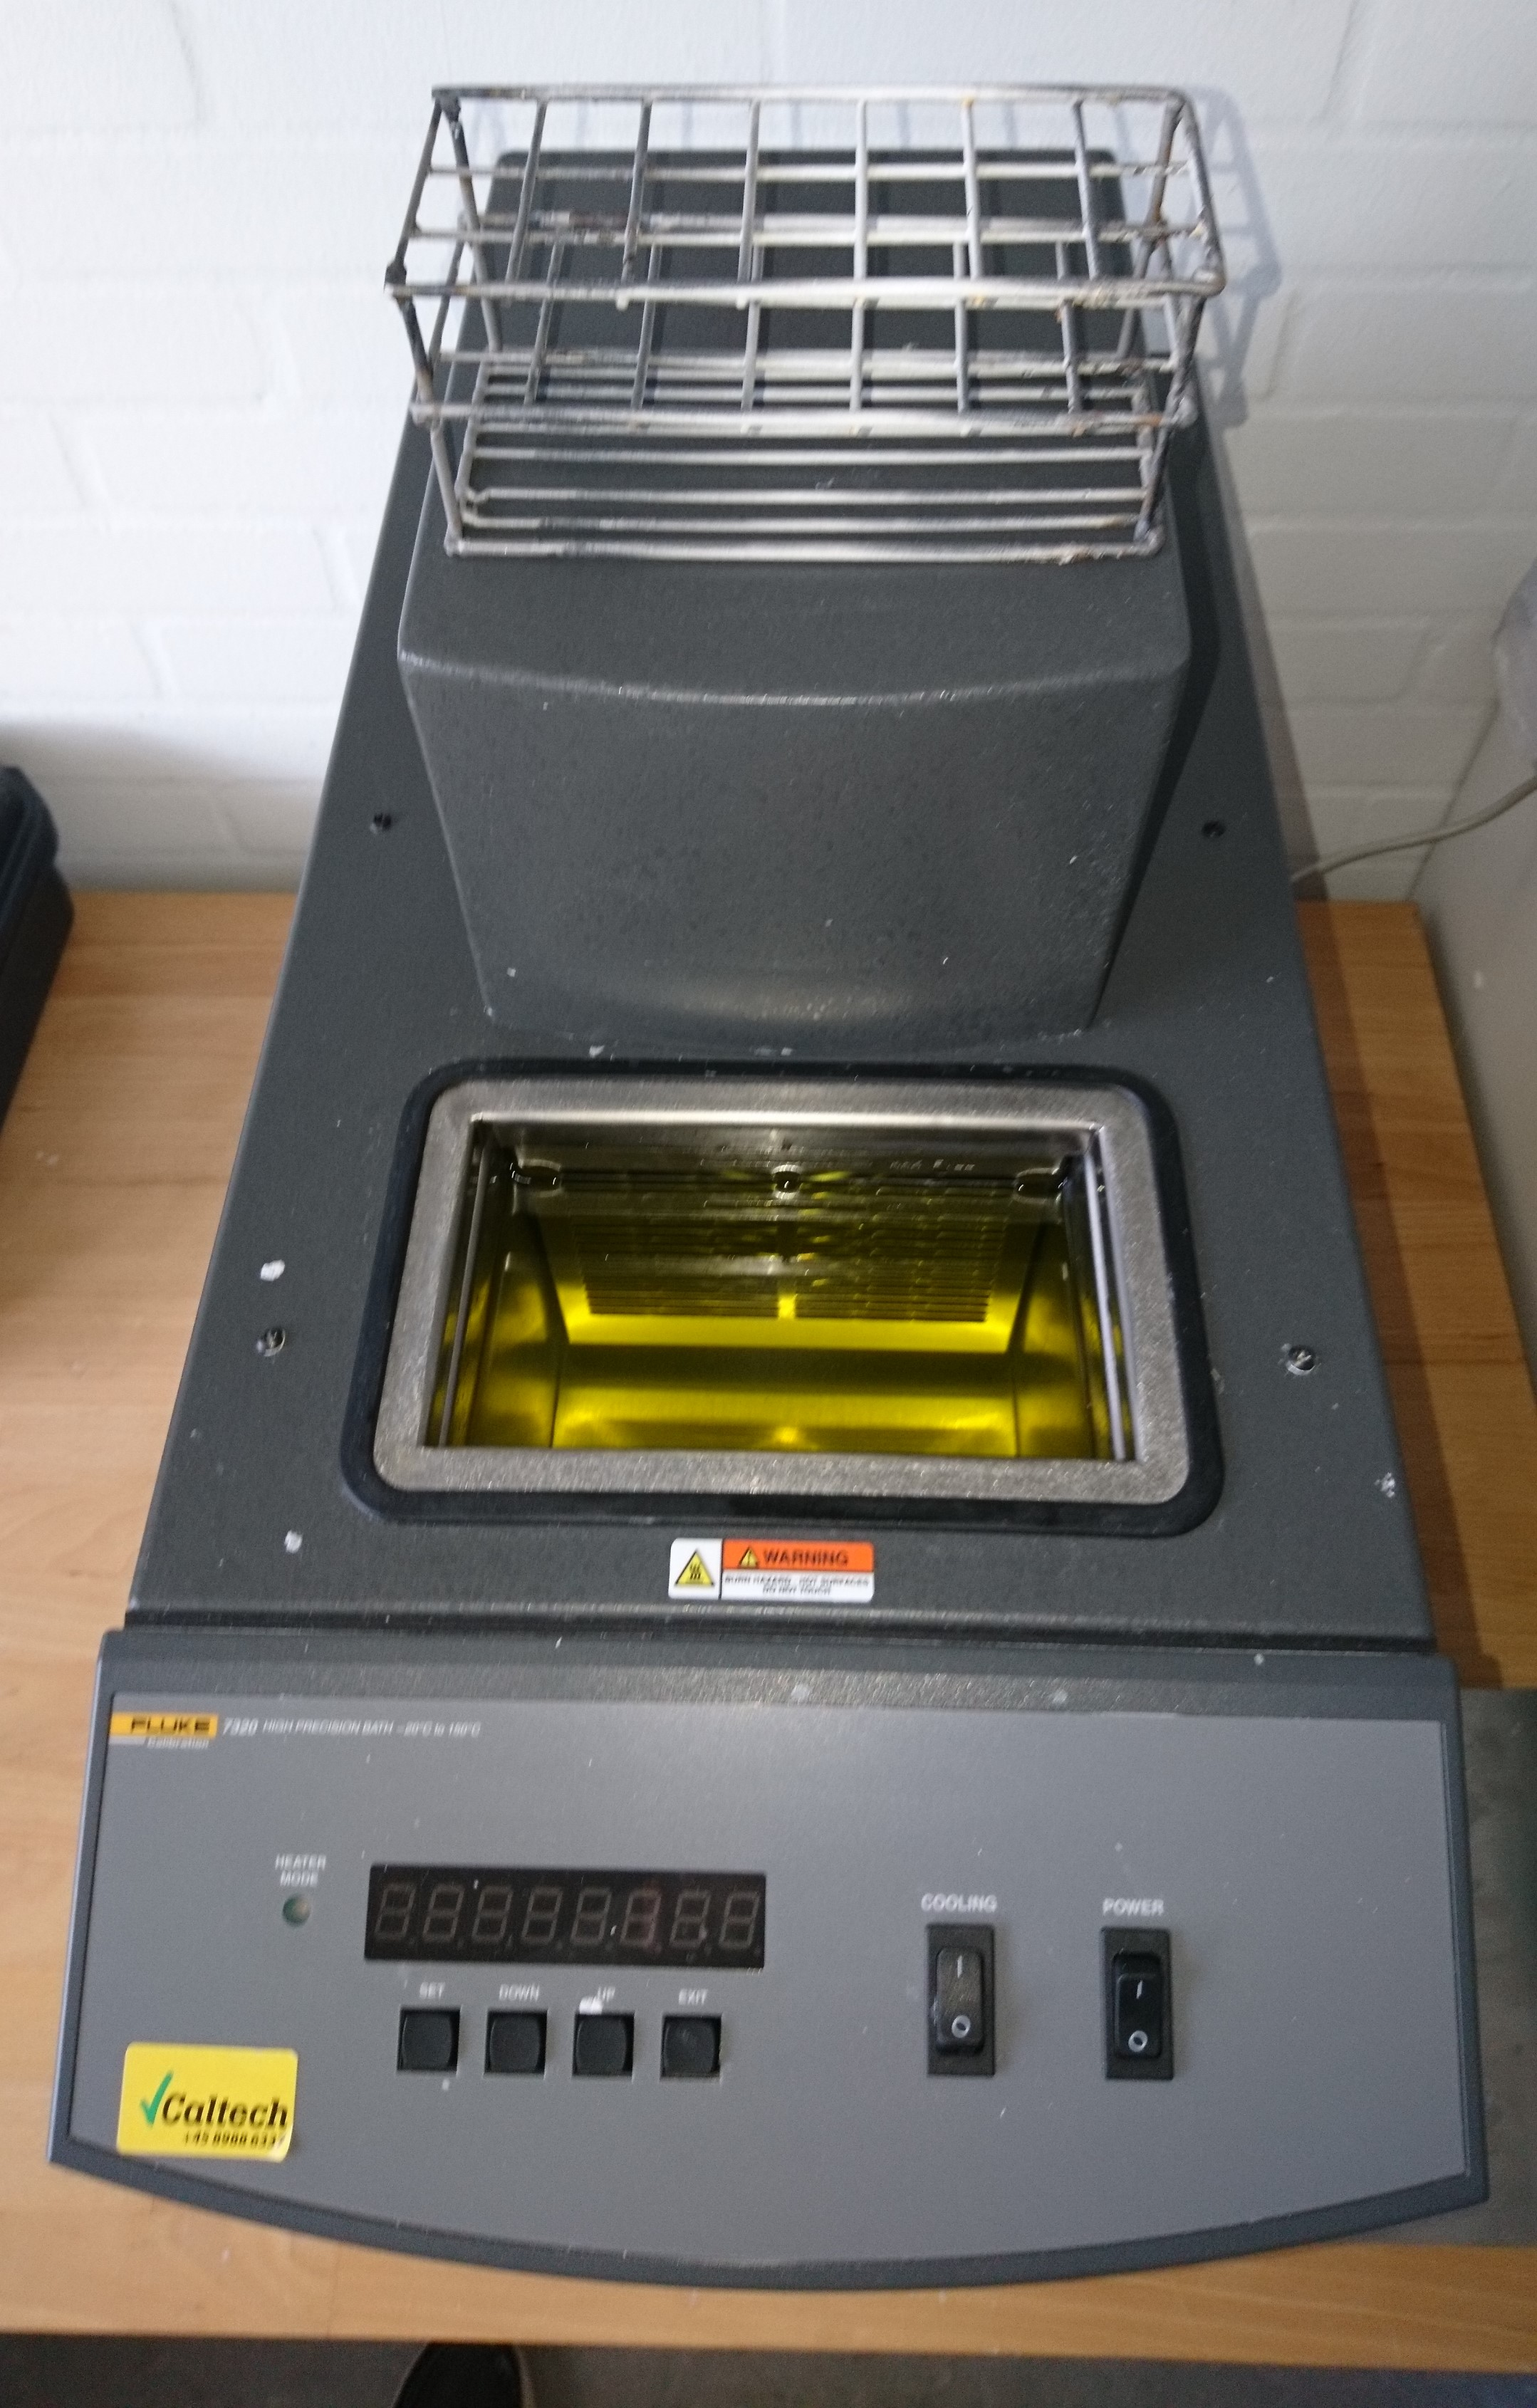
\includegraphics[width=0.3\textwidth]{kalibrerings_bad}
\caption{Det anvendte kalibreringsbad}
\label{fig:kalibad}
\end{figure}
%

Som udgangspunkt for nulpunkts kalibreringen er er "Fluke Termometer 1524" benyttet med den tynde/fleksible termistor probe. Den fejl der er på de to følere, legges til/ trækkes fra temperaturen i forsøget under resultatbehandling.
For at sikre mindst mulig forstyrrelse er dataloggeren sat til at starte målingerne efter computeren er koblet fra. For reference termometret er strømforsyningen valgt fra da den giver forstyrrelser og der er i stedet benyttet batterier.

\subsection{Forsøgsgang}
For alle målinger noteres temperatur og vægt [g], inden forsøgsstart renskes prøverne for evt. løst materiale, hvilket gøres for hånd. Derefter vejes prøven tre gange.

Vægten af isopar noteres, vægten nulstilles. Prøveholderen kommes i, derefter kommes loddet i (I+H+V), denne process (I+H,I+H+V), gentages to gange. 
Prøven kommes i, efter masse og tid er noteret tages prøven op og tørres af med papirservietter, derefter kommes holderen i, dette gentages tre gange for hvert prøveemne (I+H,I+H+P,I+H).
Efter prøven er neddykket tre gange afsluttes denne sekvens ved følgende målinger: I,I+H,I+H+V. Når en sekvens er fuldføret (en prøve) kan næste sekvens starte (prøve 2) hvor samme procedure følger. Når alle prøver er kommet i tre gange, afsluttes forsøget ved: I,I+H,I+V+H,I+H,I+V+H. For en skematisk oversigt over proceduren henvises der til bilag \vref{app:skema_ark}.

\subsection{Beregning af densitet} 
Temperatur logger og tidspunkt for målinger samkøres på den fælles tid. 
Derefter beregnes $\rho_iso$ for alle målinger med loddet, se formel 

Densiteten af Isoparens bestemmes ved at sænke et lod med kendt masse og kendt volumen ned i beholderen med Isopar, hvilket gøres to gange ved forsøgs-start og to gange ved forsøgs-slut. Hver prøve neddykkes tre gange, hvor der forinden og efter de enkelte neddykk, noteres vægten af isopar + holder. Temperaturen ved hver nedsænkning noteres, og anvednes til at samkøre temperaturmålingerne fra datalogger med de enkelte neddykkninger

Ved Arkimedes princip kan et objekts volumen bestemmes, dette gøres ved at nedsænke et legeme i en væske. Den opadrettede kraft $F_op$ (opdriften) som påvirker legeme, svarer til massen af den fortrængte væske.

Til bestemmelse af Isoparens densitet, nedsænkes et legeme med kendt masse og volumen, hvor forskellen i massen $\Delta_m$, før og efter legeme nedsænkes, svarer til volumen af det neddykkede objekt. Væskens densitet $\rho_{liq}$ bestemmes ved følgende formel \vref{eq:rho_iso}, hvor $\delta_m$ er forskellen i den noterete vægt, og $V_{obj}$ er volumen af loddet.     

%
\begin{equation}
\label{eq:rho_iso}
\rho_{I}=\frac{\Delta{_m}}{V_{obj}}  
\end{equation}
% 

De målte densiteter af isopar plottes som en funktion af den målte temperatur, og der etableres en lineær regressions linje, ud fra regressions linjens formel findes densiteten af isopar ved de målte temperaturer. 

Volumen af de enkelte prøver $V_P$ beregnes ved formel \vref{eq:vol_prove}, hvor $\Delta{m_p}$ er forskellen i den noterte vægt og $\rho_I$ er den beregnede densitet for isopar, ved den aktuelle måling.

%
\begin{equation}
\label{eq:vol_prove}
V_p=\frac{\Delta{m_p}}{\rho_I}
\end{equation}
%

%
\begin{figure}
\centering
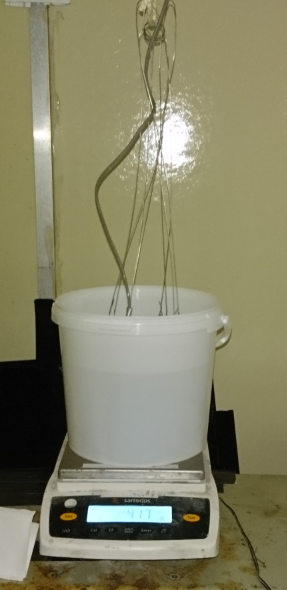
\includegraphics[width=0.30\textwidth]{ark_opst_red}
\caption{Forsøgs opstilling- Arkimedes princip}
\label{fig:ark_opst}
\end{figure}
%
\begin{figure}
\centering
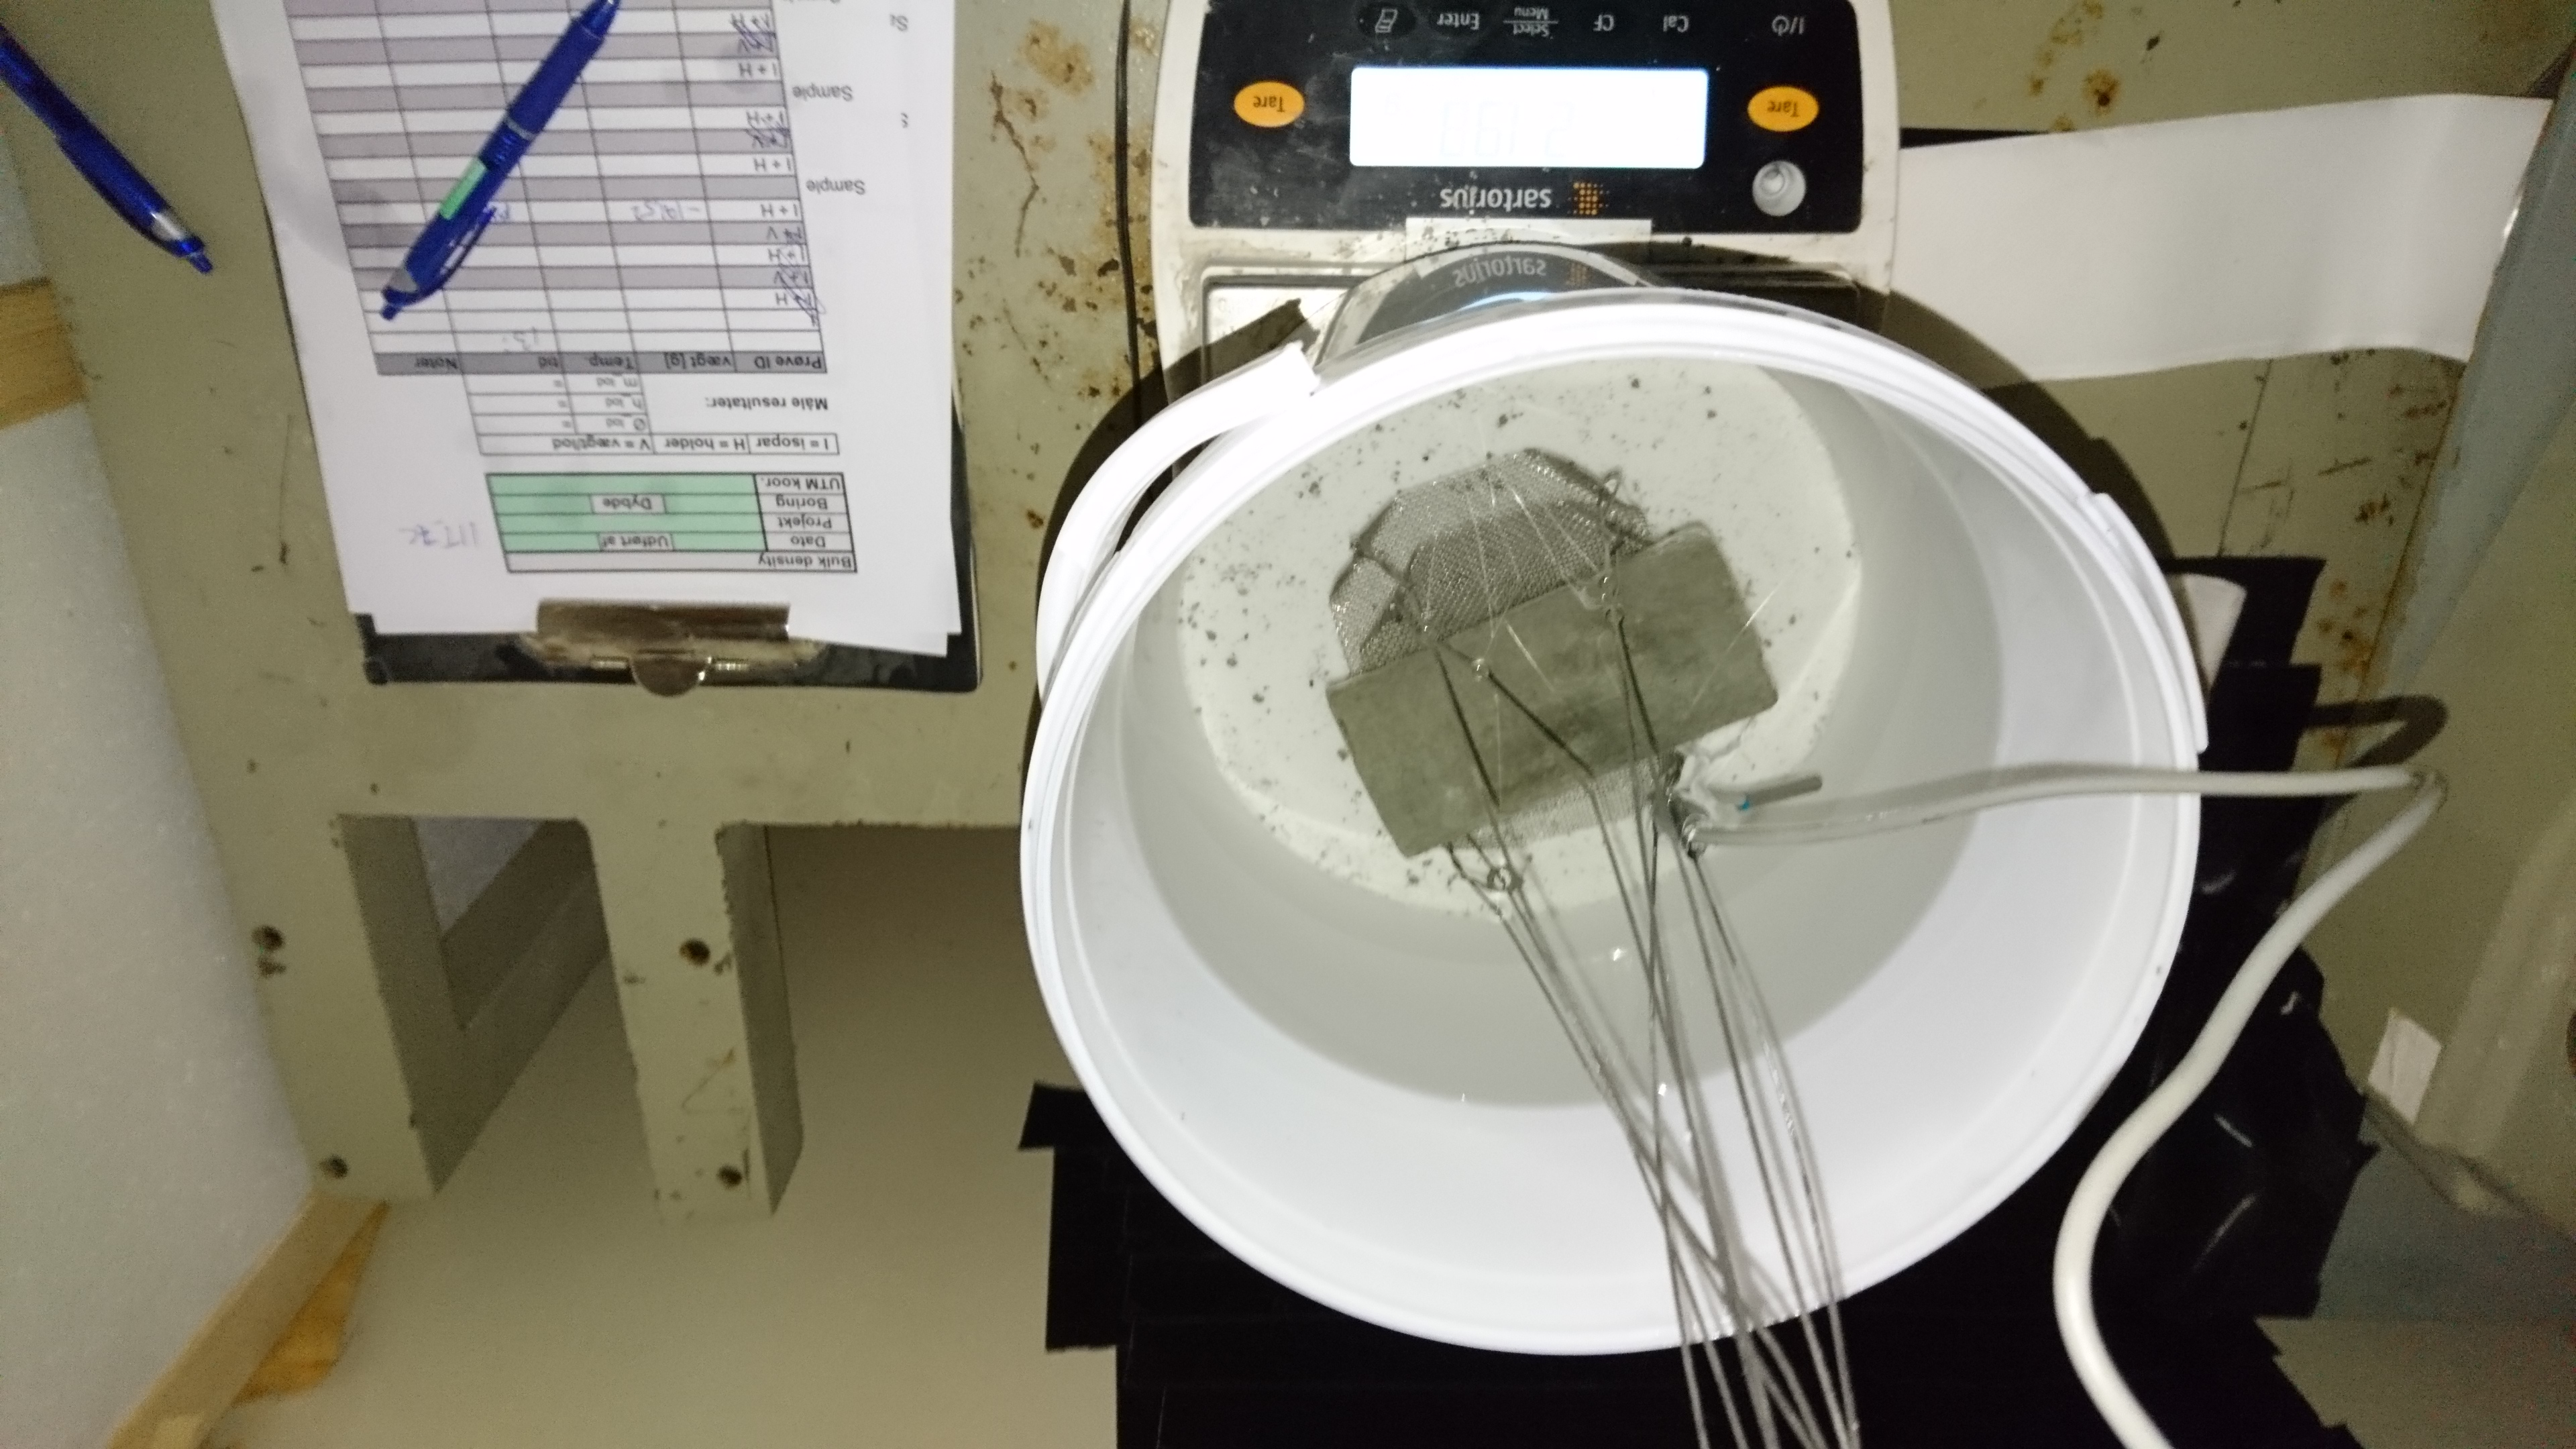
\includegraphics[angle=180,width=0.55\textwidth]{ark_prove}
\caption{Forsøgs opstilling, med prøve neddykket i Isopar}
\label{fig:ark_opst_prove}
\end{figure}
%
\paragraph{Beregning af usikkerhed}
Til bestemmelse af densiteten af isopar ved hvert enkel prøveemne anvendes en middelværdi af densiteten bestemt inden prøven nedsænkes i væsken samt den efterfølgende densitets bestemmelse. Ud gennemsnits densiteten for isopar beregnes tre volumener. Gennemsnits volumen og gennemsnits massen anvendes til at beregne bulkdensitet af prøven, ved formel \vref{eq:sd_dens}. 
%
\begin{equation}
\label{eq:sd_dens}
\frac{\sigma_\rho}{\bar{\rho}}=\sqrt[]{(\frac{\sigma_m}{\bar{m}})^2+(\frac{\sigma_v}{\bar{v}})^2}
\end{equation}
%
\paragraph{Afvigelser fra vejledning} Temperatur data fra nullpunktskalibreringen har ikke blevet behandlet, dette vil give en mindre fejl på temperaturen, isoparens densitet samt loddets volumen, dog vil det føre til en paralellforskyvning, da alle målinger vil flytte sig horisontalt langs x-axsen. Det er derfor valgt at benytte den gennemsnitlige densitet for isopar for hvert prøvemne som udgangspunkt for beregningerne, for isopars densitet plottet som funktion af temperaturen, henvises der til bilag .  så der vil ikke udgøre en forskel på beregningen af bulkdensiteten. 
